


\huge{آماده سازی داده آموزشی}\\
\large


از وبسایت وبتون\footnote{webtoon.com} چپتر هارا دانلود میکنیم و در هر صفحه OCR را اجرا میکنیم و متن هر چپتر را استخراج میکنیم و در فرمت  [chapter\_number].txt ذخیره میکنیم.
\\
از آنجایی که طبق سیاست وبسایت وبتون، تصاویر وبتون باید سایز canvas
مشخصی داشته باشد و این سایز کوچک است.
آرتیست ها روی سایز canvas بزرگتری کار میکنند
و سپس آن را برش میدهند. به همین دلیل بعضی از متن ها بین دو تصویر نصف میشوند.
برای وصل کردن تصاویر باید وجود نوشته در پایین یا بالای تصویر را تشخیص میدادیم.
برای اینکار چک کردیم در پیکسل های انتهایی، پیکسل های مشکی درون پیکسل های سفید رنگ محاصره شده اند یا نه. با این روش توانستیم تقریبا تمام متون دو نیمه شده را به هم وصل کنیم.

در قسمت تمیز کردن داده اشتباهات متدوال ocr را اصلاح کردیم.
برای مثال تعویض \$ با S
و همچنین خطوط تک واژه که اهمیتی در مدل NER ما ندارند را حذف کردیم.


سپس به کمک ابزار ntlk و تابع word\_tokenize متن را به واژه ها میشکانیم.
\\
و سپس به کمک ابزار 
spacy
جملات را تشخیص میدهیم.

\huge{برچسب گذاری}\\
\large
برای برچسب گذاری ابتدا از این وب ابزار مخصوص spacy استفاده کردیم
که متاسفانه باید کل کار را دستی انجام میدادیم و به همین دلیل خیلی زمانبر و انرژی بر بود.
 \begin{latin}
 \url{https://tecoholic.github.io/ner-annotator}
 \end{latin}
\\

و دنبال روش جدید گشتیم.
تگ های NER را از سایت فندوم وبتون \footnote{purple-hyacinth.fandom.com} crawl کردیم.
و سپس این کلمه هارا در تمام متون سرچ کردیم و index شروع و پایان با تگ مورد نظر 
را در فایلی به نام train\_data.json ذخیره کردیم.

تعداد جملات قبل تمیز شدن و برچسب گذاری: 9540

تعداد جملات بعد تمیز شدن و برچسب گذاری: 1177


\huge{آمار داده ها}\\
\large



أ. تعداد «واحد» داده , ب. تعداد جملات
\begin{latin}
\begin{center}
  \fontsize{8pt}{9pt}\ttfamily
  \csvautotabular[respect all]{../stats/sentences_count.csv}
\end{center}
\end{latin}

\\

ج. تعداد کلمات
\begin{latin}
\begin{center}
  \fontsize{8pt}{9pt}\ttfamily
  \csvautotabular[respect all]{../stats/words_count.csv}
\end{center}
\end{latin}

\\

د. تعداد کلمات منحصر به فرد

\begin{latin}
\begin{center}
  \fontsize{8pt}{9pt}\ttfamily
  \csvautotabular[respect all]{../stats/unique_words_count.csv}
\end{center}
\end{latin}


\newpage

و.  ۱۰کلمه پرتکرار غیر مشترک هر برچسب
\begin{latin}
\begin{center}
    \fontsize{4pt}{7pt}\ttfamily
  \csvautotabular[respect all]{../stats/ten_dissimilar_words.csv}
\end{center}
\end{latin}

ز. ده کلمه مشترک برتر براساس relative normalized frequency
\begin{latin}
\begin{center}
    \fontsize{4pt}{7pt}\ttfamily
  \csvautotabular[respect all]{../stats/relative_normalized_frequency.csv}
\end{center}
\end{latin}


ط. هیستوگرام تعداد تکرار هر کلمه منحصر به فرد به ترتیب از فرکانس بالا به پایین
\begin{figure}[H]
    \centering
    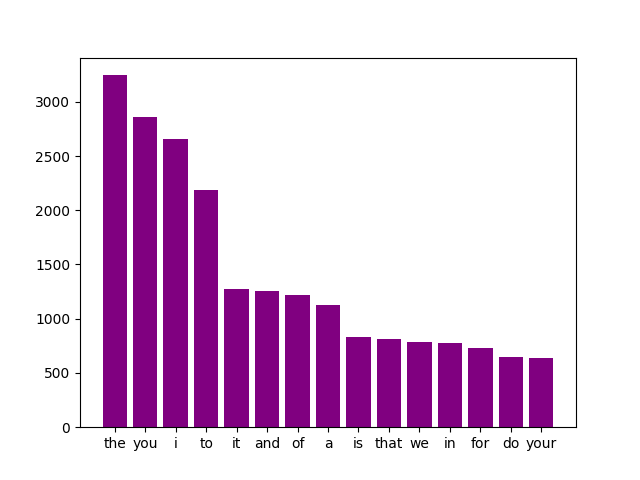
\includegraphics[width=0.7\linewidth]{../stats/hist.png}
   \end{figure}
   
لینک \lr{github} :

 \begin{latin}
 \url{https://github.com/Bayany/NLP_NER}
 \end{latin}

لینک \lr{huggingface}:
 \begin{latin}
\url{https://huggingface.co/datasets/Bayany/NER}
 \end{latin}
 
